%************************************************
\chapter{`Bee Watching'}
%************************************************
\begin{flushright}
March 7, 2013
\end{flushright}
\section{Prior Aim}
	To study the co-relation between the flower colour and bee flower selection. Figure out if the flower colour affects the behaviour of bees?
\section{Motivation}	
	In plants, we observe either self-fertilisation/pollination or cross fertilisation. Insects play an important role in the pollination process for certain plants.
	\par
	Behaviour of Pollinators in general depends on, visual cues and olfactory cues. The plants `allegedly' use colour and fragrance to attract pollinators and `reward' them in return for pollination, with nectar and pollen (these are eaten to gain lipids).

\section{Proposed Techniques}
	The following are the techniques can be employed:
	\begin{enumerate}
		\item Focal Animal Sampling: \par
		In this method all occurrences of the specified action of one individual are recorded for a predetermined interval of time.
		\item Activity Scans: \par
		An individual's activities are recorded at regular intervals, for example, every 30 seconds.
		It provides the percent of time spent in a particular activity. Instantaneous scan sampling is best done with a sample interval as small as possible and an easily identifiable behaviour. 		
	\end{enumerate}
	In this experiment we used the method of focal animal sampling.


\section{Procedure}
	The procedure was as follows:
	\begin{enumerate}
		\item Located a suitable region, viz. a region with multiple coloured flowers of the same species
		\item Ensured the pollinators we're about to follow are bees and not `copycats'
		\item Started an audio recorder
		\item Narrated suitably the actions of one bee for as long as possible
		\item Repeated the procedure for over 6 bees and 2 regions
	\end{enumerate}

\section{Analysis}
	\subsection{Brief of the Statistics}
	Too see if the difference in the average duration is statistically significant, we perform a two tailed t test as the sample size is extremely small and the t-test depends only on the the degrees of freedom of the system being analysed. If we can relate our means and variances with this distribution, it becomes simply a matter of looking up values to find the probability of their occurrence, assuming the Null hypothesis to be true. We now define a less than $5\%$ probability of occurrence to mean that the means are too different to belong to the same population, and thus the null hypothesis must be rejected. 
	We've found experimentally, $m_1$, $m_2$, $s_1$, $s_2$, $n_1$ and $n_2$, which are means, variances and degrees of freedom respectively.
	We find the t value using the following equation
	\begin{equation}
		t=\frac{m_1 - m_2}{\sqrt{\frac{s_1^2}{N_1} + \frac{s_2^2}{N_2}}}
	\end{equation}
	Also, we find the degrees of freedom, given by
	\begin{equation}
		df = (N_1 -1) + (N_2 -1) = (N_1 + N_2 -2)
	\end{equation}
	Now all we have to do is look up the value in a t-table corresponding to $0.050$ and $df$ as calculated. If $t_\text{calculated}>t_\text{table}$, then the Null hypothesis is rejected. Else, the null hypothesis can not be rejected.


	\subsection{Implementation}
		The basic idea here is to find out if there's a co-relation between the flower colour and bee flower selection. Our method is, as stated earlier, focal animal sampling. So we have to do the following multi-stage analysis to get the desired result. We analysed this data on excel, and the commands used have been casually hinted at for reconstruction should the need arise.
		\begin{enumerate}
			\item Collected the raw data and converted it into a table, `CroppedCollected' with the headings `Bee Number ID', `Colour of Flower' and `Time Spent on Colour', ensuring that each bee was followed for roughly the same period of time.
			\item Using a Pivot Table, converted `CroppedCollected' into a table that gives the total time spent on each colour, in a given Time Sample (viz. for a given bee). The table was then converted to an ordinary table, with fields `Bee Number (ID)', `Colour of Flower' and `Sum of Duration', given in \autoref{bee_data_fixedtime}
			\item Next converted this into a Pivot table with `Colour of Flower' in the Rows, and in the Values, `Average of the Sum of Duration' and `Count of Flower'. The corresponding graph for this is given in \autoref{bee_cropped}.
			\item On the basis of this graph, categorized the `Colours' to a `Family' and created a table for the same. \autoref{bee_table_category}
			\item Using this final table, created another Pivot Table with Rows `Family' and Values were `Average of Sum of Duration', `StdDev of Sum of Duration' and `Count of Flower'. The data is given in \autoref{bee_final}
		\end{enumerate}

\section{Result}
	We can't reject the Null Hypothesis, viz. The bees select between the different colour families randomly.

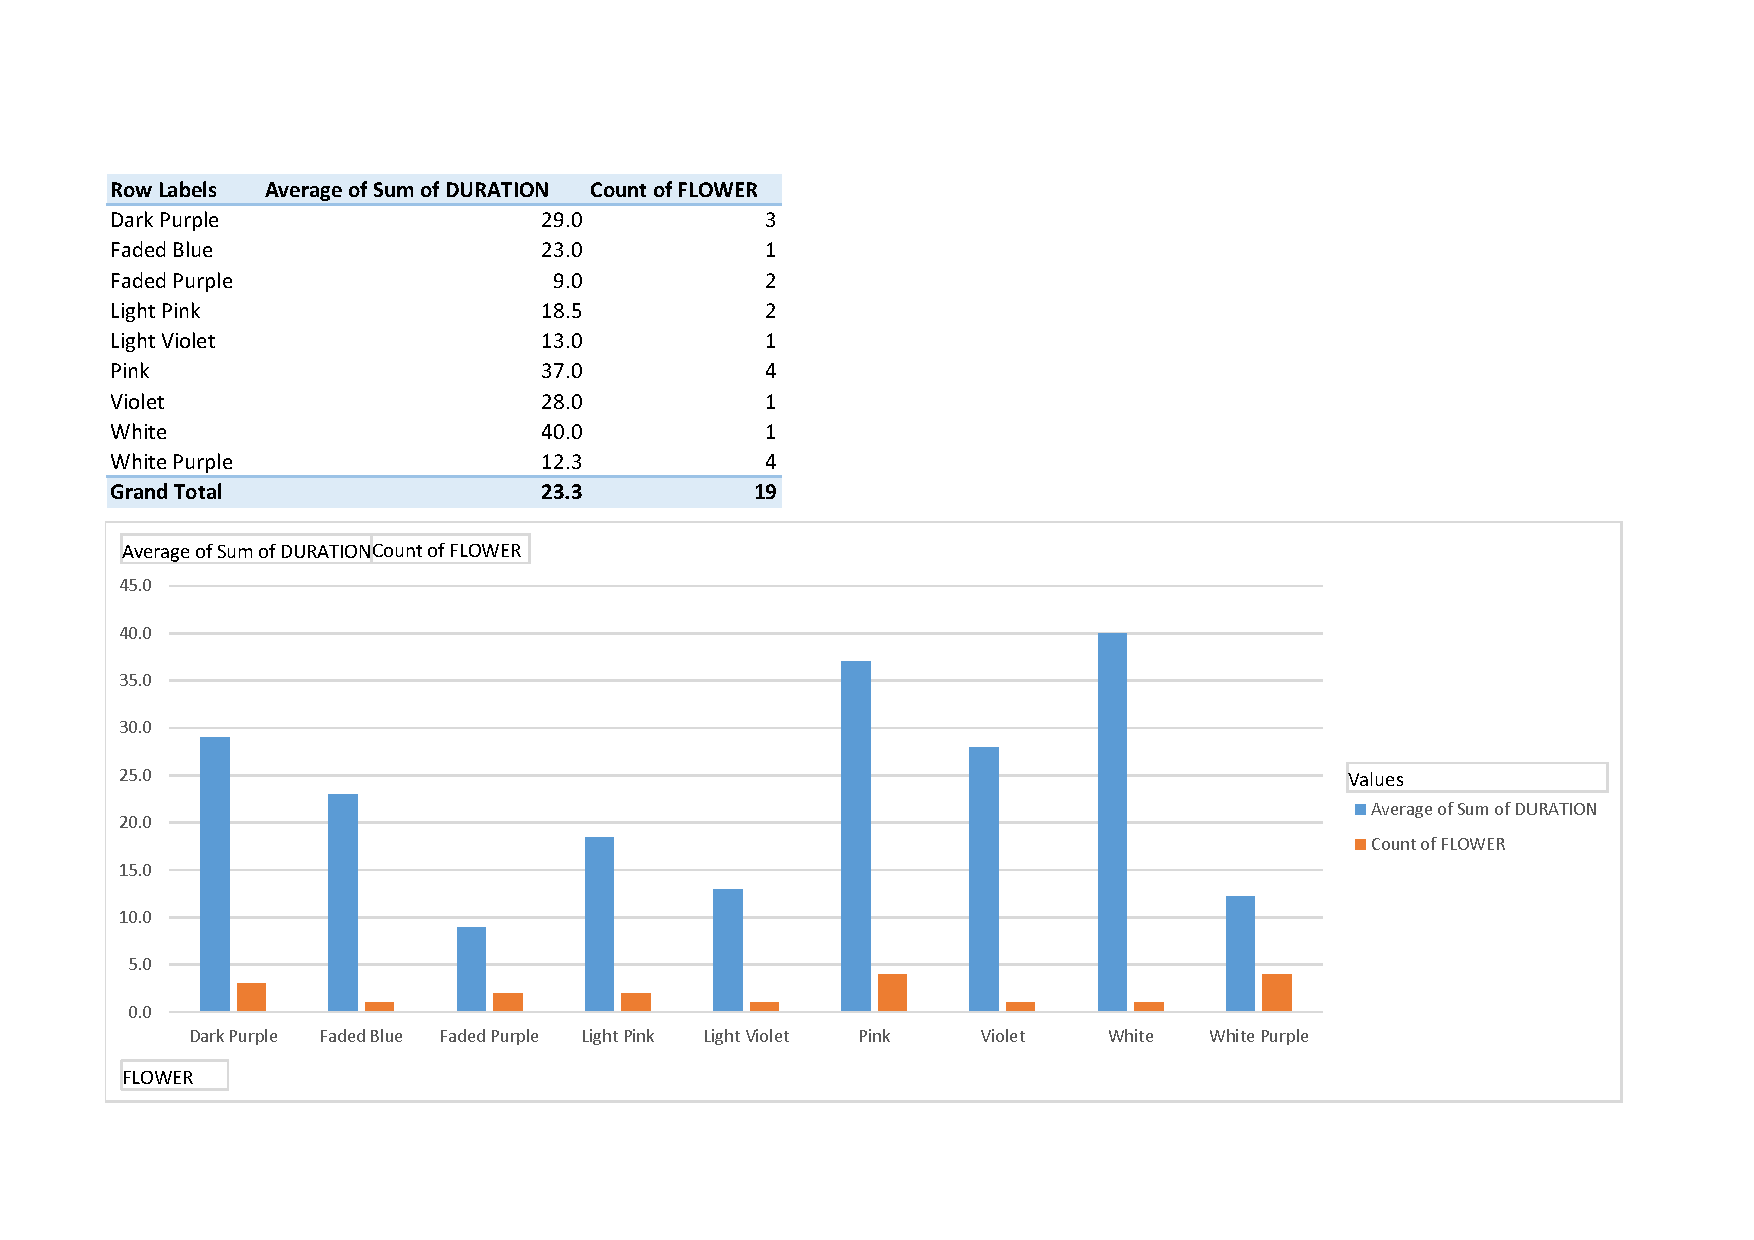
\includepdf[pages=1-,addtolist={1,table,{Bee Data Cropped},bee_cropped},pagecommand={\pagestyle{empty} \autoref{bee_cropped}}]{gfx/bee/ritu_table_main.pdf}

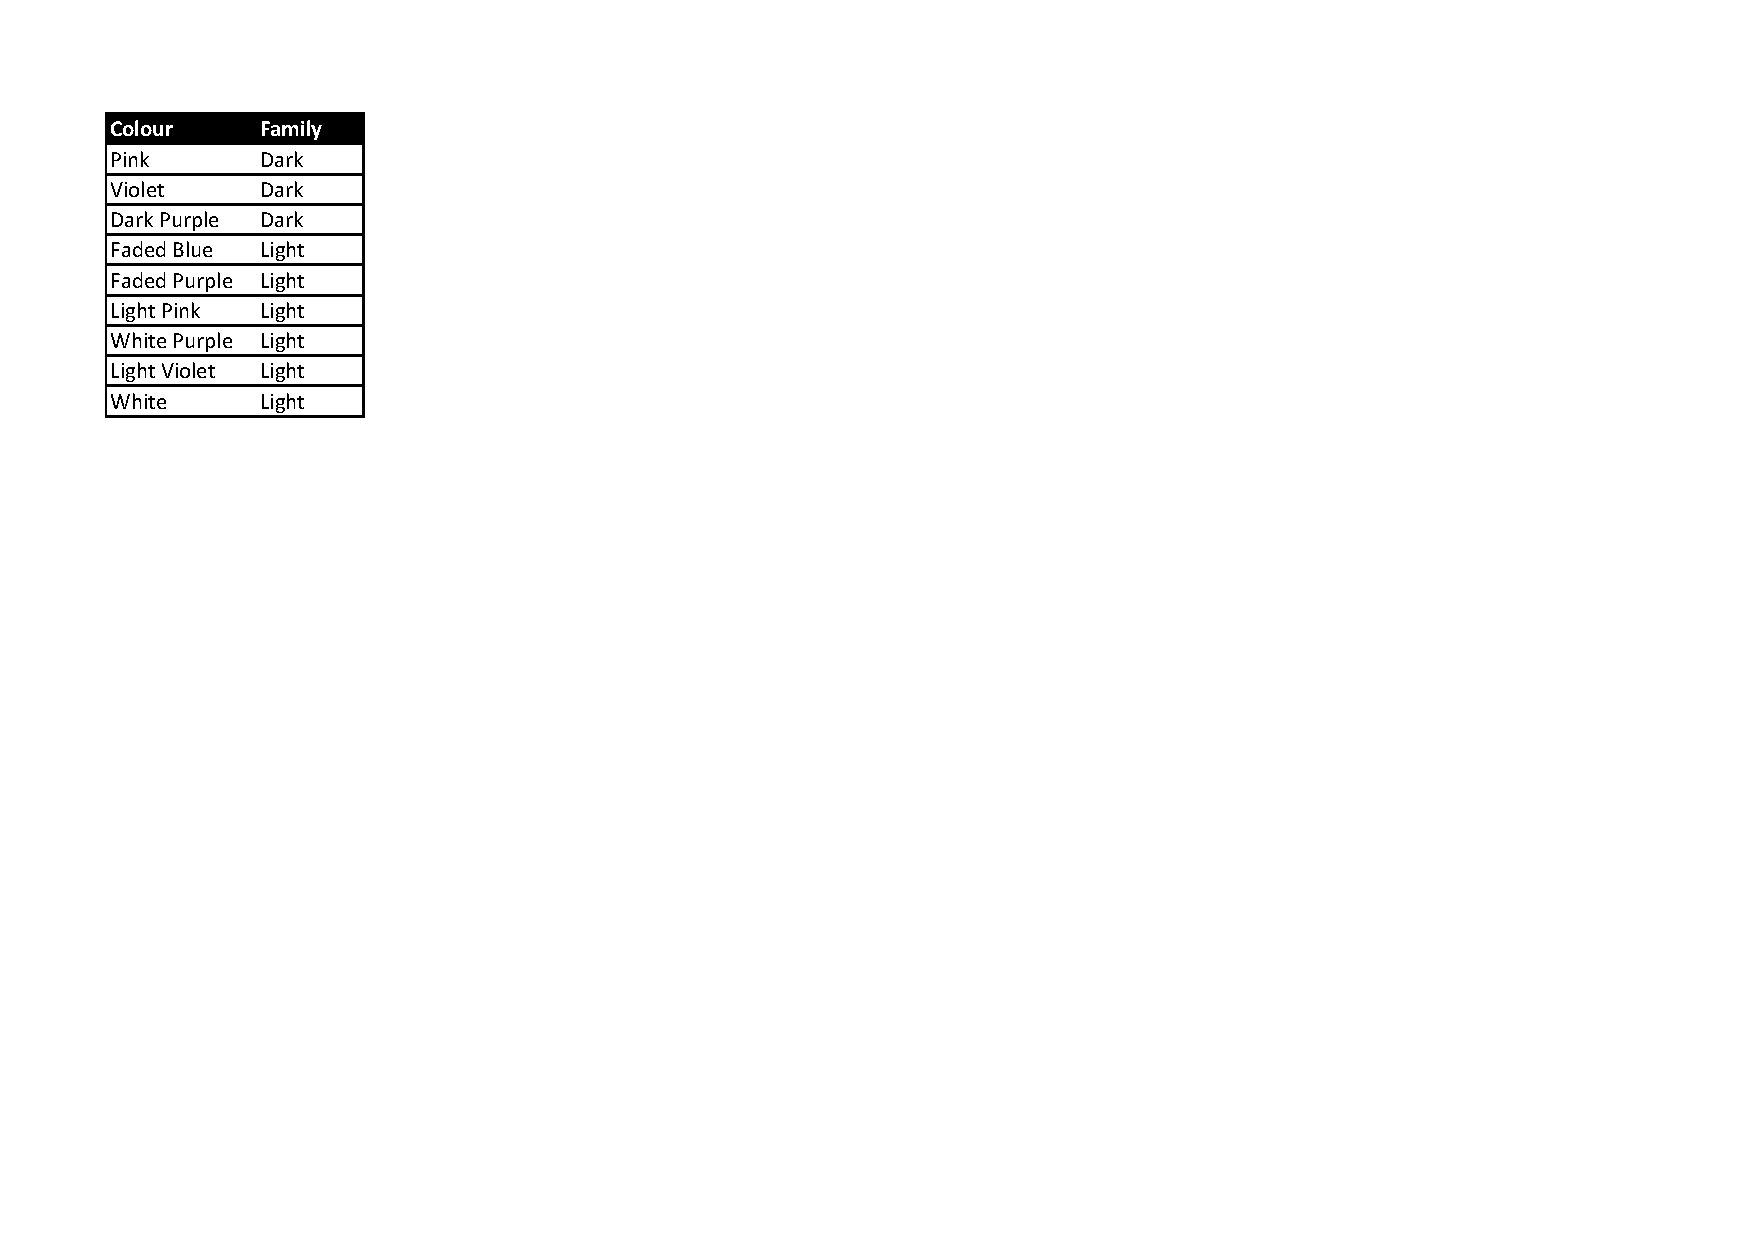
\includepdf[pages=1-,addtolist={1,table,{Colour Family},bee_table_category},pagecommand={\pagestyle{empty} \autoref{bee_table_category}}]{gfx/bee/ritu_table_category.pdf}

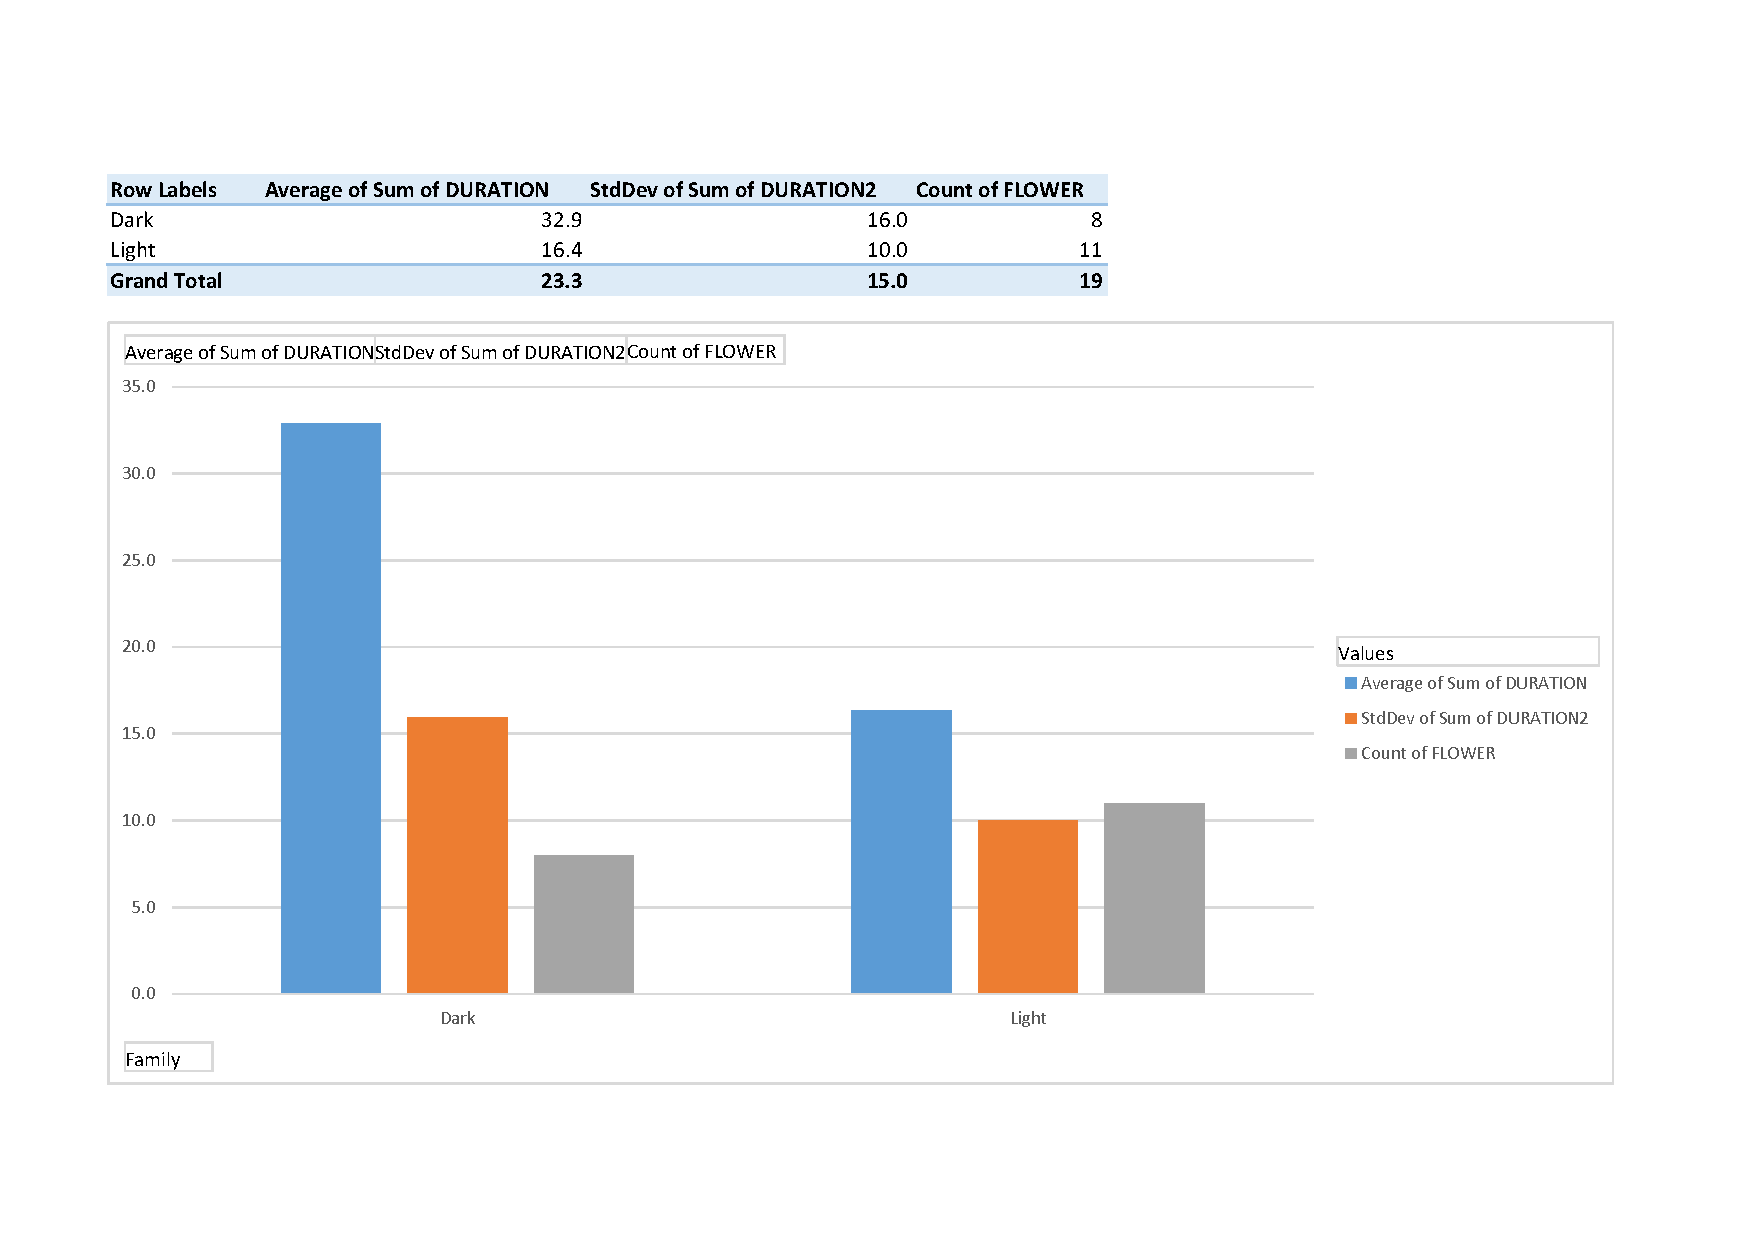
\includepdf[pages=1-,addtolist={1,table,{Colour Family},bee_final},pagecommand={\pagestyle{empty} \autoref{bee_final}}]{gfx/bee/ritu_final.pdf}

% \section{Precaution}

% \section{Acknowledgements}	